\documentclass{article}
\usepackage{graphicx}
\usepackage{geometry}
\usepackage[left=1in,right=1in]{geometry}                
\usepackage{amssymb}
\usepackage{amsbsy}
\usepackage{amsmath}
\usepackage{multirow}
\usepackage{lineno}
\usepackage{caption}
\usepackage{longtable}
\usepackage{setspace}
\usepackage{fancyhdr}
\usepackage{natbib}
\usepackage{subfigure}
\usepackage{booktabs}
\usepackage{lscape}


\graphicspath{ {graphs/} }
\title{Dan Looks at Flowers and Leaves, and Tries LaTeX for the very first time}
\author{Dan Buonaiuto}
\date{}

\geometry{legalpaper,  margin=1in}

\usepackage{Sweave}
\begin{document}
\begin{flushleft}
Dan Buonaiuto\\
December 2016
\end{flushleft}
\begin{center}
\Sconcordance{concordance:flobudgraph_page.tex:flobudgraph_page.Rnw:%
1 26 1 1 0 40 1}

\section*{Do Flowers and Leaves phenophases respond to the same proximate cues? }
\end{center}

In indivudual plants, do flower and leaf bud respond to the same envrionmental cues to intiate spring phenophases? This is unknown, because flowering and leafing phenology are rarely studied to gether. As global climate changes, so too, does phenology. If floral and foliate pheenophase are initatied by the same cues, their sequences and temporal patterning should stay relatively fixed in relation to each other, responding to climate change in accordance. If, however, floral and foliate phenophases are resonding to different cues, the floral-leaf phenological sequence may become uncoupled, which could have fitness consequences, eg. loss of hysteanthy.\\
\\
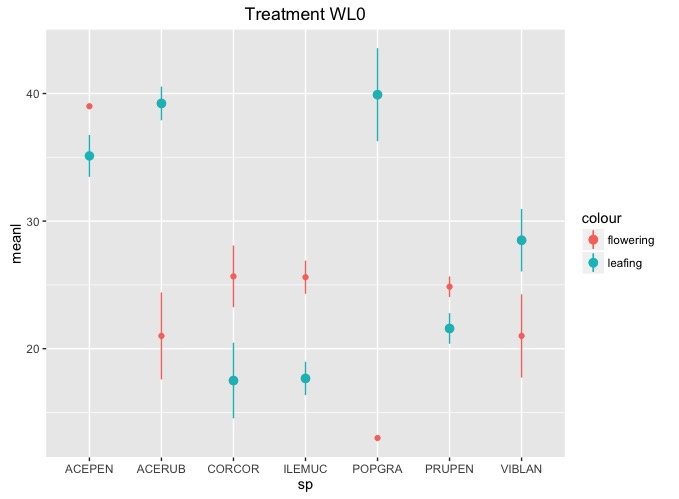
\includegraphics[width=9cm] {WL0}
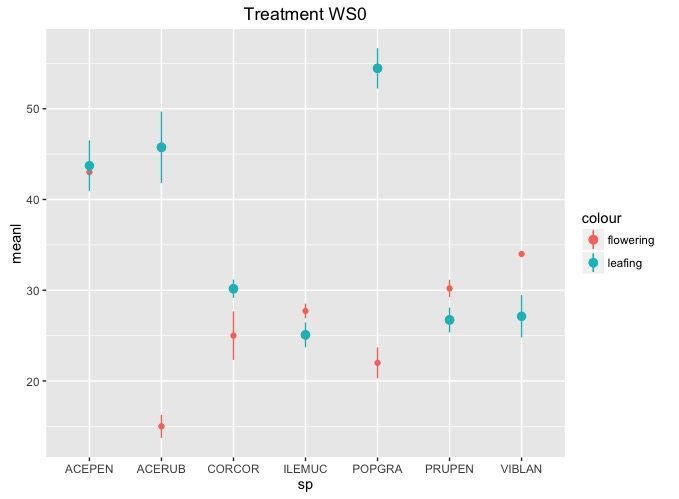
\includegraphics[width=9cm]{WS0}\\
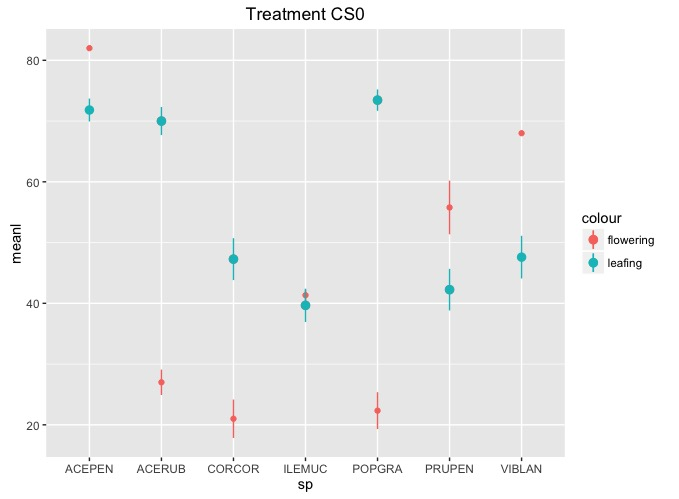
\includegraphics[width=9cm]{CS0}
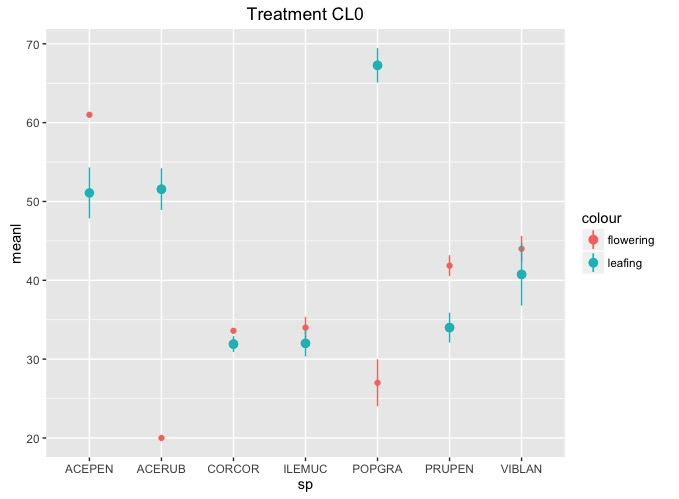
\includegraphics[width=9cm]{CL0}

These graphs are somewhat interesting. It does seem like in some of the species, flowering and leafing are responding differently to the treatments. Until I learn sweave, for a more clear rendering of the graphs, see the "graphs" folder in the "Flo buds" subsection of bud on github. However this might just be a sampling artifact. As you can see in the table below, data for flowering were extrememely poorly represented. Only \textit{Prunus pensylvanica, Corylus cornuta} and \textit{Ilex mucronata} had even slightly adaquate flowering--interesting that they are all shrubs.
\begin{center}
\begin{table}[h!]{}
\rezsizebox{5in}{!}
\begin{tabular}{||c| c c |c c |c c| c c||}
\hline
 &WL0& &CS0& &WS0& &CL0&\\
 \hline
&	Flowered&	Leafed&	Flowered&	Leafed	&Flowered	&Leafed&	Flowered&	Leafed\\
\hline
ACEPEN	&1&	9&	1&	11&	1&	11&	1&	12\\
ACERUB	&2&	9&	4&	10&	2&	8&	2&	9\\
CORCOR	&9&	10&	5&	11&	3&	12&	5&	11\\
ILEMUC	&5&	12&	6&	12&	7&	12&	6&	12\\
POPGRA	&2&	11&	3&	9&	2&	11&	2&	11\\
PRUPEN	&7	&12	&9	&12	&5	&11	&7	&12\\
VIBLAN	&2	&8	&1	&10	&1	&8	&2	&8\\
\hline
\end{tabular}
}
\caption{The number of observations of flowering and leafout by species per treatment}
\end{table}
\end{center}
\end{document}
